\chapter{Estado da Arte} \label{cap:eda}
%2345678901234567890123456789012345678901234567890123456789012345678901234567890

Preliminarmente...

Falar aqui o que é ontologia, porque isso é importante e como jogos ou a
industria de entretenimento pode ver isso como util.

\section{Modelo Cognitivo Emocional} \label{cap:eda:mce}

Estudos neurológicos recentes \cite{ledoux1998emotional,damasio2004erro}
mostram a importância das emoções na tomada de decisão. A emoção é definida
como um estado físico do corpo e o sentimento é a percepção desse estado
corporal \cite{damasio2004erro}. Além disso, na psicologia há diferentes
modelos que tentam explicar a afetividade.

\citet{scherer2000tnoe} categorizou esses modelos afetivos em quatro
categorias principais. A primeira categoria, modelos dimensionais, visa
descobrir variáveis que representam eixos das classes emotivas e estabelecem
meios de se mover por esses eixos. Os modelos discretos especificam um
conjunto básico de emoções e especificam regras para que o mecanismo evolua.
Já, a categoria dos baseados em significados se preocupa com as situações
em que o sentimento foi ocasionado e tenta descrever estruturas semânticas dos
mesmos. Por fim, os modelos baseados em componentes entendem que os
sentimentos são aprendidos ao longo do tempo e, sendo assim, estudam o elo
entre os sentimentos e as suas situações. Esse elo é montado de diferentes
formas e varia de pessoa para pessoa.

\begin{figure}[t]
  \centering
    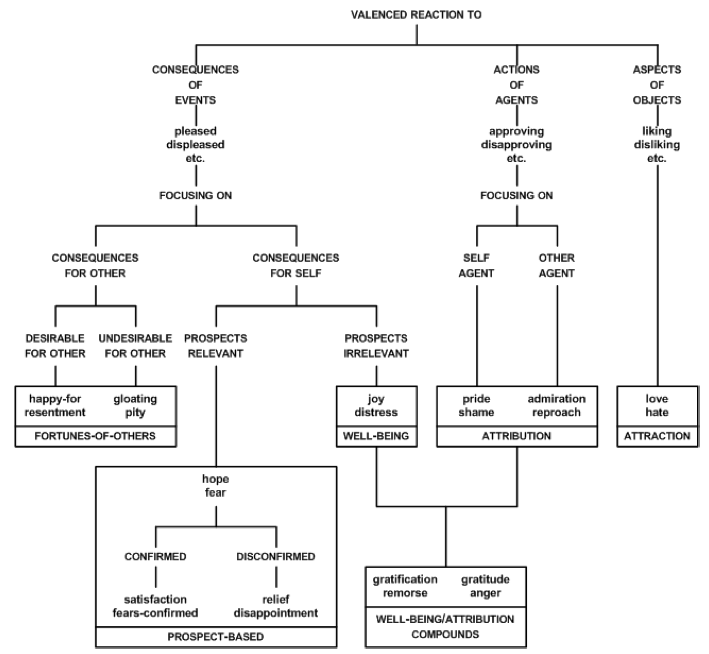
\includegraphics[width=150mm]{figuras/occ.png}
  \caption{Estrutura de emoções \cite{ortony1988cse}.}
  \label{fig:occ_model}
\end{figure}

Um modelo bastante conhecido na Inteligência Artificial foi definido por
\citet{ortony1988cse}. Esse modelo baseado em 
significados por descrever as situações de ocorrências de cada uma de suas 22
emoções.  Essas emoções são divididas em formas de se perceber o mundo a sua
volta por consequências (importantes para alguma meta), responsabilidade (pode
se auto julgar) e atração (ou repulsa). Assim sendo, essas maneiras de se
perceber o mundo refletem diferentes jeitos de se analisar as situações que
podem ser relativas aos objetivos, valores morais ou gostos da pessoa.

A Figura~\ref{fig:occ_model} resume esse modelo e mostra as
percepções possíveis de um indivíduo.  Partindo da direita para esquerda, o
ramo mais básico, Aspectos de Objetos, é ativado quando se avalia o gosto de
alguém para algum objeto (inanimado ou não). Por exemplo, alguém gostar de
rosas vermelhas.  No seguinte, Ações de agentes, o julgamento das ações
exercidas por outro indivíduo é realizado baseado nos valores morais da pessoa
que está julgando. Exemplo: reprovar a atitude de um colega que ``colou'' no
teste. O último ramo da árvore, mais a esquerda, é o de consequências de
eventos que representa as coisas que aconteceram (e foram consideradas
importantes), acontecem ou acontecerão (objetivos almejados)\dev{}. Essas
emoções são avaliadas segundo as consequências para o alcance ou impedimento
dos objetivos de uma pessoa. Exemplos desse ramo pode ser a emoção sentida
ao receber uma boa nota em um teste ou, ainda, receber um agradecimento.

Toda a emoção do modelo trabalha com duas intensidades. A intensidade da
emoção que representa o físico e a intensidade do sentimento que representa o
quanto o agente esta percebendo daquela emoção. Dessa forma, um indivíduo só
possui sentimento quando a intensidade da emoção ultrapassa um
determinado\dev{}
limite.  Essa intensidade é obtida por uma função matemática que utiliza
variáveis de dois tipos: local, que influência as emoções do ramo específico;
e global, que influência todas as emoções do modelo.  Um exemplo de variável
local é o desejo, enquanto que um exemplo de variável global pode ser o senso
de realidade.

\citet{bates1994role} afirmou que o comportamento emotivo de um personagem é
um papel importante para ser ter a ilusão de vida. Esse trabalho foi um dos
primeiros à utilizar o modelo descrito visando melhorar a credibilidade de
seus atores ligando cada uma das emoções com um determinado tipo de
comportamento. Por exemplo, um agente liga o medo a um comportamento agressivo
enquanto outro liga essa mesma emoção com um comportamento retraído.

Com a finalidade de demostrar que as emoções melhoraram a credibilidade dos
atores, \citet{zhang2009emotional} desenvolveram uma aplicação. Nesse
trabalho, os sentimentos afetam a forma que o planejamento das ações é
realizado. \citet{neto2010construction} visaram entender o impacto da emoção
na tomada de decisão. Assim, eles fizeram com que agentes pudessem
``esquecer'' determinadas crenças quando o estado emocional fosse diferente
daquele guardado anteriormente. Essa característica torna o planejamento e as
atitudes dos personagens virtuais mais realistas.

O objetivo de \citet{bick2003relational} com o projeto \emph{Relational
Agents} é possibilitar aos usuários a criação de um relacionamento social e
emocional com longa duração.  Em \citet{bickmore2009virtual}, a confiança no
agente tornou possível discutir tarefas mais importantes como melhoria da saúde
ou até a compra de uma casa. Da mesma forma, o projeto
AIDA\footnote{Mais detalhes, ver http://senseable.mit.edu/aida} (do
inglês \emph{Affective Intelligent Driving Agent}) pode ser entendido como
enquadrado na área de Interface Homem Computador, pois o interesse é entender o
estado afetivo da pessoa dirigindo. Além disso, o agente pode tentar sugerir
ao usuário mudanças em suas rotas baseado na rotina aprendida anteriormente.

\section{Ontologias Emocionais} \label{cap:eda:oe}

Aqui tem que ter pelo menos 5 ontologias explicadas;
%1
%2
%3
%4
%5


\section{Ontologias de Humanos Virtuais} \label{cap:eda:odhv}

Explicar...
	pq ela eh necessaria.
	pelo menos 2.
%1
%2
